
\documentclass[16pt,twocolumn,letterpaper]{article}
\usepackage{apacite}
\usepackage{tablefootnote}
\usepackage{titling}
\usepackage{graphicx}
\usepackage[T1]{fontenc}
\usepackage{babel}

\usepackage{titlesec}% http://ctan.org/pkg/titlesec
\titleformat{\section}%
  [hang]% <shape>
  {\normalfont\bfseries\Large}% <format>
  {}% <label>
  {0pt}% <sep>
  {}% <before code>
\renewcommand{\thesection}{}% Remove section references...
\renewcommand{\thesubsection}{\arabic{subsection}}%

\setlength{\droptitle}{-12em}  
\setlength\bibitemsep{\baselineskip}
\title{Experimenting with Scaleable Forecasting Models}

\author{
    Matthew Coghlin\\
  	\and
  	Pelumi Dacosta\\
    \and
    Joseph Despres\\
    \and
    Aneesh Gahi\\
    \and
    Joseph Sigler\\
}

\author{ Matthew Coghlin, Pelumi Dacosta, Joseph Despres, Aneesh Gahi, Joseph Sigler}

\begin{document}

\maketitle
\bibliographystyle{apacite}


\section{Introduction}

Planning organizational activities such as inventory planning, staffing decisions, budgeting, all depend on an expected future value. Forecasting the practice of using current data available to make a prediction about the future a variable at a time that has not yet happened. Decision makers in government, businesses, and non-profit organizations all require accurate and reliable forecasts when planning their various activities. There are tremendous costs associated with forecasts that are either too high or too low. Therefore, as practitioners, it is essential to minimize forecasting error. 

Organizations are collecting more and more data as it becomes cheaper to store and more convenient to collect. This presents the opportunity to use more data driven forecasts and less judgment based forecasts. For accurate, reliable, and interpretable forecasts a time-series expert is generally required to carefully tune model parameters \cite{taylor2018forecasting}. Although, this approach is riggerois, it does not scale, any standard grocery store has more items to overwhelm anyone manually tuning models. Analysts could be asked to generate high quality forecasts for thousands, and even hundreds of thousands of series at a time. The goal of this project is to implement forecasting algorithms that generate high quality forecasts with minimal involvement, validate them with a training and testing partisan, and generate ensemble predictions made up of the various predictions.

\section{Data}

The data obtained for this project are provided as part of a Kaggle challenge where participants are to forecast daily retail sales demand \cite{kaggle}. As contestants, we are given 5 years of training data, with the daily sales of 50 different products from ten different stores. This is a total of 913,000 data points to train forecasting models. The goal is to forecast the next 90 days for each of the 50 products and 10 stores. Judged by Symmetric Mean Absolute Percentage Error (SMAPE) shown in Equation 1

\begin{equation}
\textrm{SMAPE}={\frac {100\%}{h}}\sum _{t=1}^{h}{\frac {\left|\hat{y}_t-y_t\right|}{(|y_t|+|\hat{y}_t|)/2}}.
\end{equation}

where $y_t$ is the actual value, $\hat{y}_t$ is the forecast, and $h$ is the forecast horizon. This metric is used the account for the different magnidudes of many series to give a fair comparasent. Should you simply use Mean Absolute Percentage Error, there is an asymmatry as forecasting low is penalized more than forecasting high as well as errors in a series with a lower number of units \cite{hyndman2006another}.

The data required very little preparation. There were several data points that were zero we switched to a one because the one of the algorithms did not support 0 values. After that we combined the stores and items into one string column to avoid nesting loops when iteration over stores and items. Notice Figure 1 shows data are highly seasonal with a slight upward trend and substantial noise.

After that, we separated into training and testing partisans to get an idea of what kind of model performance we can expect. We selected the first 1279 data points or 80\% training set of our time-series. Then we separated the remainder of the data as a testing set. This prepares us for running the experiments.

\begin{figure}[!htb]
	\center{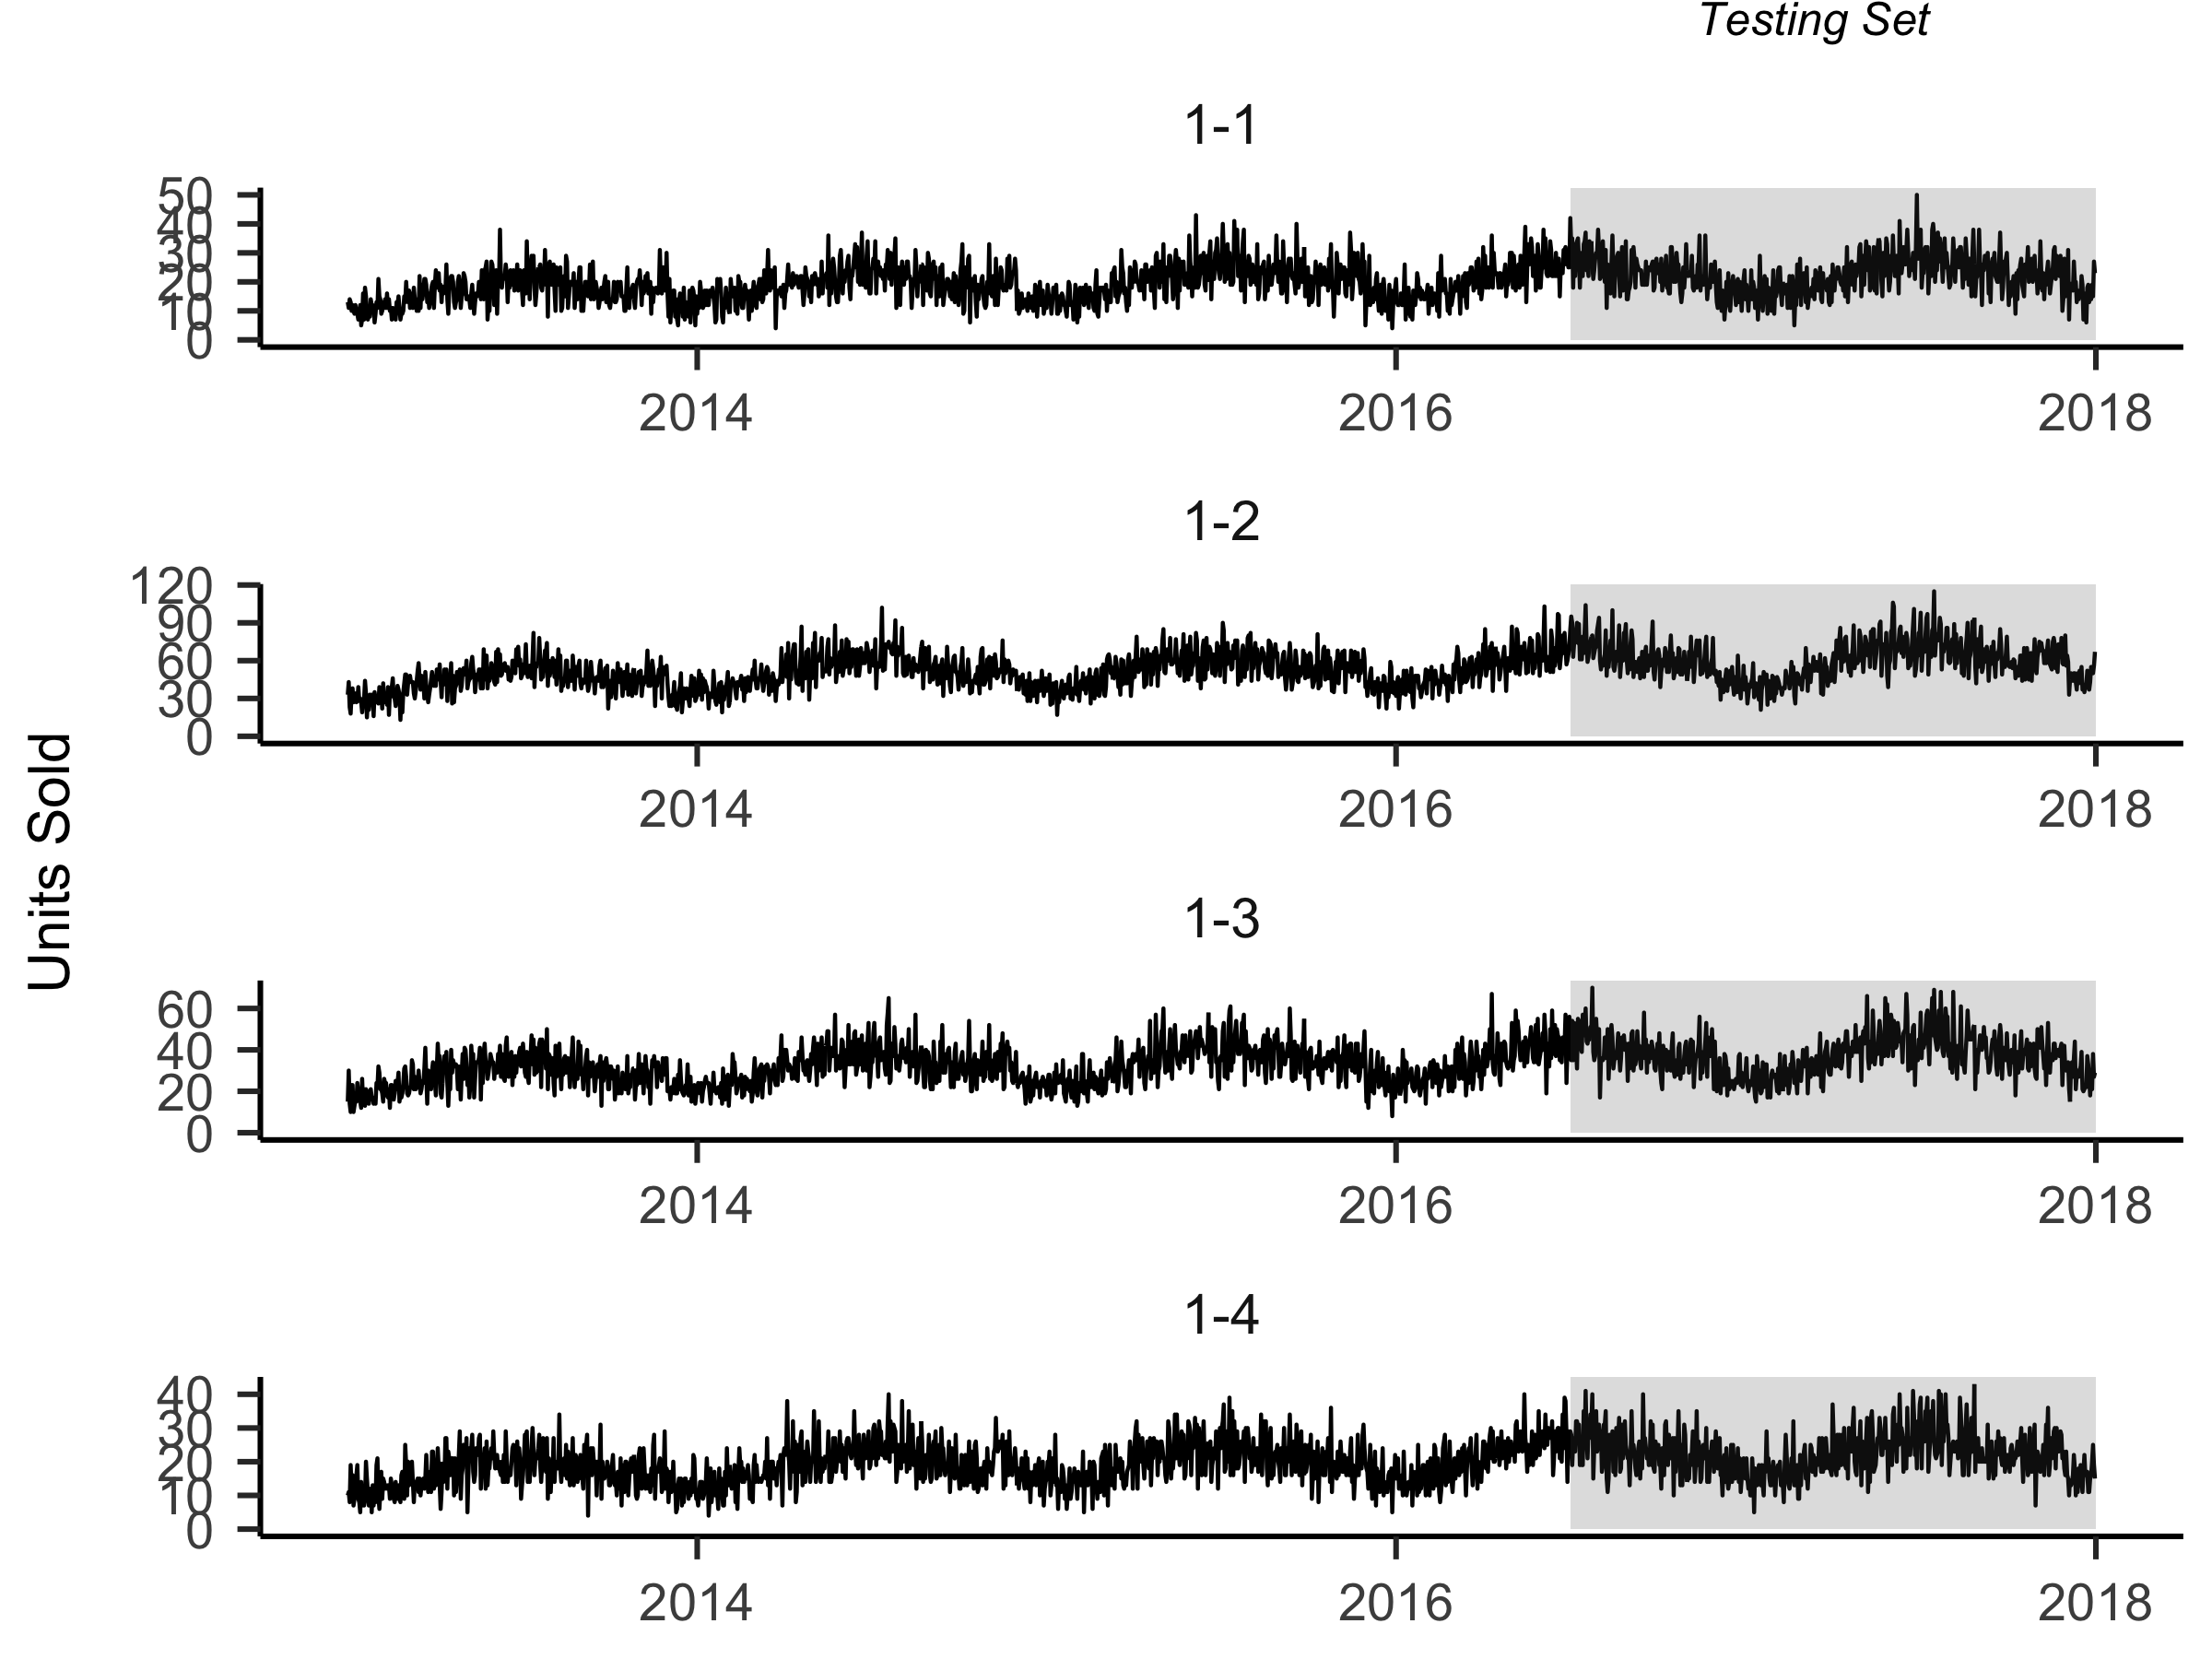
\includegraphics[width=\columnwidth]
        {plots/item_sales.png}}
	\caption{\label{fig:my-label} Daily Sales of the First Four Items in the First store}
\end{figure}

\section{Requirements}

Selecting algorithms to generate high quality forecasts will have strict requirements. These need to be fast, accurate, and interpretable. To be fast, the models must have minimal parameters to tune or be accurate with some specified default parameters. Grid searching model parameters over many series is not feasible. If these alogrythms are fast, many can be ran. Therefore, you can have a very good idea of what kind of performance to expect. Due to the high costs associated with forecasting errors, these models must be interpretable in the event a steakholder is undertain about the model. For obvious reasons, stakeholders should not be asked to place their faith in black-box forecasting models.

\section{Models}

There are many forecasting models, however we selected models that have been shown to perform well in practice and fit our project requirements. We choose to test two categories of models. First, classical models that have been successfully implemented with years of good results. They are derrived with statistical methods and have strong theoretical justifications. Second, are newer machine learning based models. This is an open field and we are going to test different models and evaluate them strictly on their performance on testing data. 

\begin{enumerate}
\item Seasonal Exponential Smoothing
\item Vector Autoregression
\item Autoregressive Distributed Lag
\item XGBoost 
\item Prophet
\item Neural Prophet
\end{enumerate}

\subsection{Seasonal Exponential Smoothing}

The Seasonal Exponential smoothing model, sometimes known as the Holt-Winters method, decomposes the timeseries into three components: Linear Seasonality, Linear Trend, and Gaussian noise \cite{hyndman2018forecasting}. This is a simple, interpretable model, that is fast to impliment and has proven quite reliable.

\subsection{Vector Auto Regression}

The first algorithm we implement, is an autoregressive model. This takes the first 5 lag positions and uses them as regressors, then using timeseries decomposition, it models the seasonality\cite{hamilton1994}. This model is commonly used to forecast economic variables.

\subsection{Auto Regressive Distributed Lag}

ARDL models add to the above auto regressive model, however in addition to seasonality with is fit with a vector of indicator variables. and trend, in this case we are adding an explanatory variable of time and fitting the model to laggs of time.

Although there are many forecasting models to choose from, there is not much research on when a given forecasting model outperforms another. Due to the data having strong weekly swings, we implement several models with an autoregressive terms.


\subsection{XGBoost}

XGBoost is an implementation of a tree boosting system. This uses decsision tree regression, and fits an ensamble of models fit to the data, then the residuals, then fits the residuals residuals. This ensamble of tree boosting is quite robust and is useful for a variety of different regression and classification tasks.

\subsection{Facebook's Prophet}

Facebook released a forecasting library designed specifically to meet the challenges of generating many high quality forecasts. The model prophet is a General Additive model, that consists of three functions, trend which fits an aperiodic logistic population growth model (we did not limit the growth, however that is a parameter), seasonality is a fouire series fit to the remaining seasonal component, and a holiday parameter which is a vector of user specified holliday periods, the holliday periods saw a drop in sales, however not enough to justify us specifying specific dates. 

\subsection{NeuralProphet}

NeuralProphet, is a forecasting library that expands on facebook prophet and includes an autoregressive term in the general additive model and uses neural networks to generate the autoregressive terms in the model \cite{triebe2021neuralprophet}.

\section{Performance}

Althoguh the Kaggle challenge is asking for a daily sales forecast, we are going to cover aggregated forecast performance because stakeholders are often far more concerned with weekly or monthly forecasts than daily. The selected forecasting models varied in performance quite dramatically. See Table 1 the the SMAPE of each model. First, we speak to the validity of each model given the performance on these testing data. Although there are 500 series, this is retail sales demand and it exhibits similar patterns. Of the selected models Facebook's prophet outperformed the rest at each level of aggregation. This is not surprising as it is percicely designed for the task of forecasting at scale \cite{taylor2018forecasting}. As the level of aggriagation increases, we observe lower errors. 

An advantage od the large volumne of forecasts gives a pretty good idea of the level of performance to expect from these models. Table 2 contain histograms of the testing set predictions. With six forecasting models forecasting a testing set fo 

\begin{figure}[!htb]
	\center{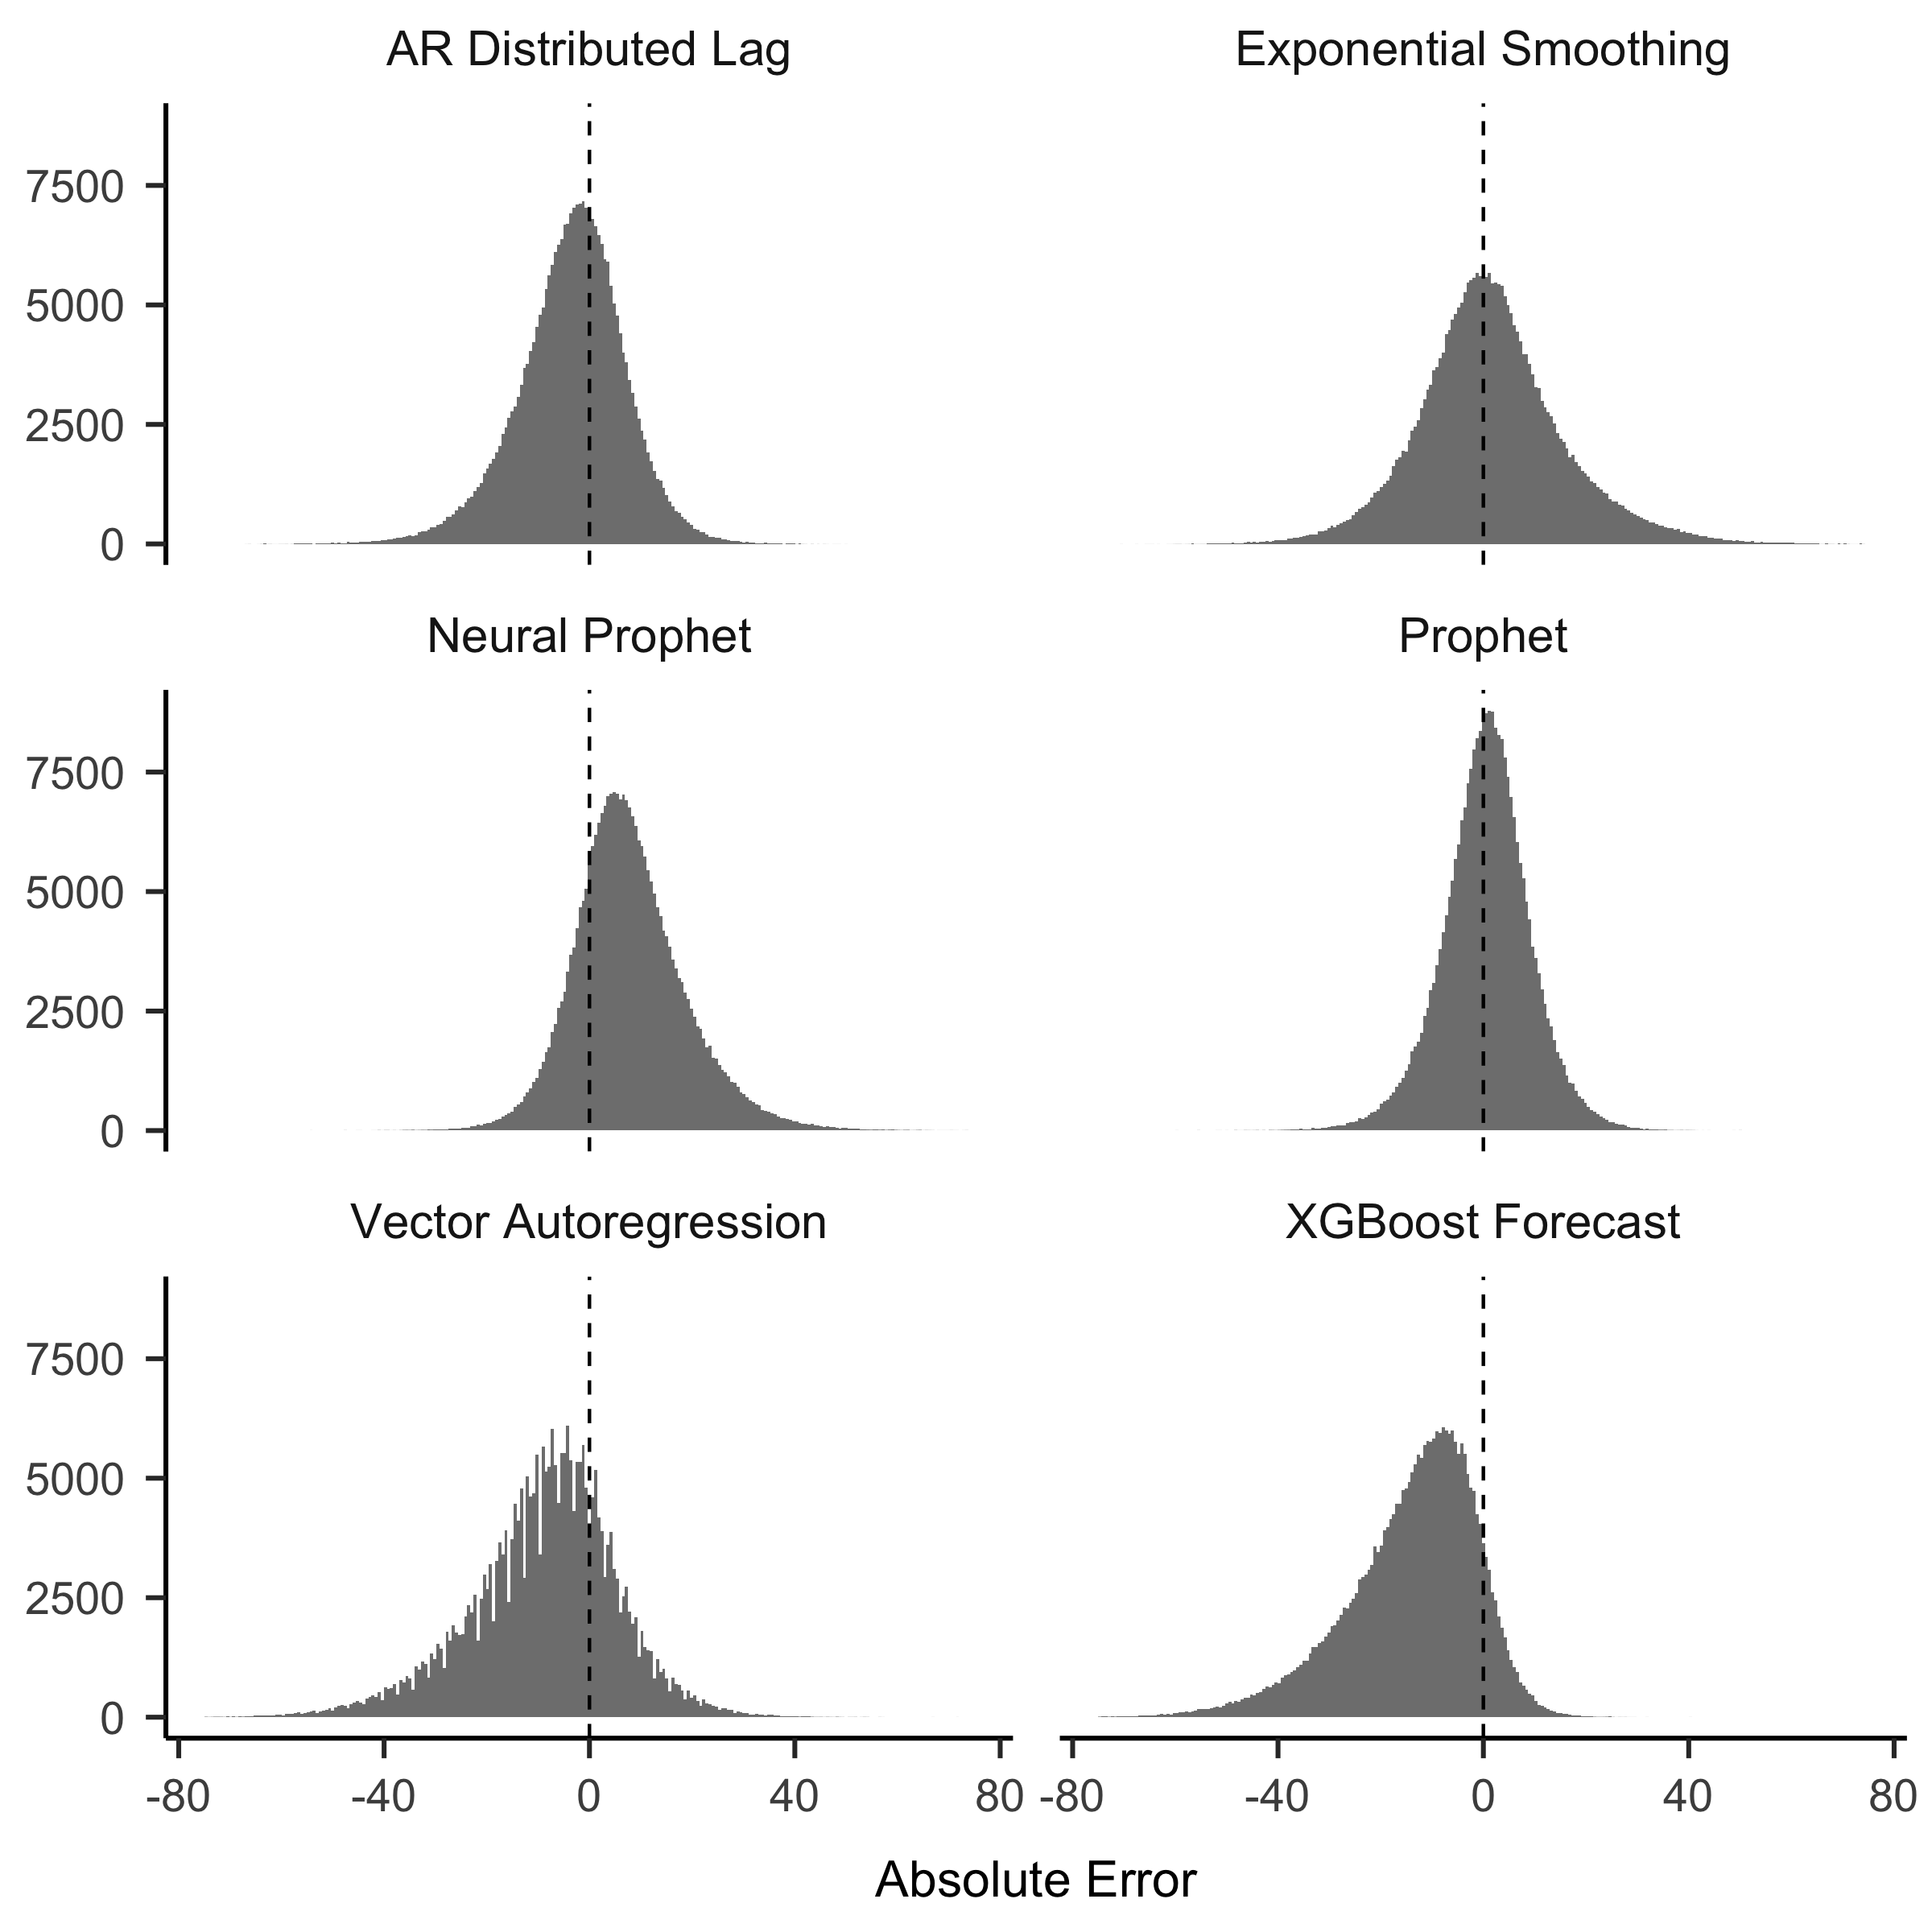
\includegraphics[width=\columnwidth]
        {plots/errors.png}}
	\caption{\label{fig:my-label} Distribution of forecasting errors}
\end{figure}



\begin{table*}[t] 
\centering 
\caption{Testing Set Forecasting Model Performance} 
\begin{tabular}{@{\extracolsep{5pt}} lccc} 
\\[-1.8ex]\hline 
\hline \\[-1.8ex] 
Model & Daily Forecast & Aggregated Weekly & Aggregated Monthly \\ 
\hline \\[-1.8ex] 
Facebook's Prophet & $12.89$ & $7.33$ & $4.24$ \\ 
ARDL & $16.83$ & $8.94$ & $4.48$ \\ 
Neural Prophet & $18.44$ & $10.46$ & $7.61$ \\ 
Exponential Smoothing & $19.31$ & $14.88$ & $13.54$ \\ 
Autoregression & $23.93$ & $17.51$ & $16.25$ \\ 
Xgboost & $30.35$ & $28.85$ & $28.43$ \\ 
\hline \\[-1.8ex] 

\footnotesize{Measured SMAPE in See Equation 1}\\
\end{tabular} 
\end{table*}



\section{Kaggle Challenge}

Feature Detection

There are many different shapes and patterns a timerseries plot can take. Tsfeatures \cite{montero2020fforma} quantifies different features such as the number of times it crosses the median, degree of seasonality, the number of flat spots, entropy, and many more. 

We ran this algorythm on each series collecting 30 quantified features. The central question of this study is to determine if we can determine which forecast will perfrom the best given these features. 

Predict Which Day the Model Has the Smallest Error Given the Features

Using different models, we tried knn, logistic regression, XGBoost, and an artificial neural network. 

Due to the way kaggle scores, final Predictions could not be a weighted average of the results. We selected which was most likely to be the final.


\section{Conclusions}

The models ensamble was able to outperform each of the individual. In practice, it is likely that we are too use these methods to forecast a months sales. this would be aggrigated.

\clearpage
\onecolumn

\bibliography{References}

\end{document}